%!TeX root=./thesis.tex

\chapter{Active Learning}
\label{cha:active-learning}

In this chapter we discuss active learning and look at its application to both
the galaxy classification task and to the Radio Galaxy Zoo project.

\section{Introduction}
\label{sec:intro-active-learning}
    
    In supervised learning we deal with a set of data points and their
    associated labels. This dataset may be expensive to obtain, but the main
    costs may come from collecting labels, rather than from collecting the data
    points themselves. Examples of such data include text samples
    \citep{lewis94, mccallum98}, and images \citep{loy11, lintott08}, both of
    which are now widely and cheaply available through the internet. A more
    abstract example is scientific hypotheses \citep{king04}. Labelling text and
    images is hard, error-prone, and requires humans; and performing a
    scientific experiment to test a hypothesis is considerably more expensive
    than coming up with the hypothesis. It may even be the case that we simply
    cannot label all the data because there is too much, such as in the Galaxy
    Zoo \citep{lintott08} and Radio Galaxy Zoo \citep{banfield15} projects.

    \emph{Active learning} (or \emph{query learning} \citep{settles09, seung92,angluin86})
    allows a machine learning algorithm to select specific, unlabelled examples
    to be labelled by an expert. The algorithm effectively chooses its own
    training set \citep{settles09}. The hope is that the algorithm can choose to
    label only the most useful examples \citep{mccallum98}, and the expensive
    process of labelling redundant or useless examples is avoided
    \citep{engelson99}. Intelligently selecting the training set as in active
    learning can result in massively reduced labelling costs \citep{lewis94,
    king04} or even make intractable labelling problems tractable.

    While there are many variations of active learning scenarios, we focus on
    \emph{pool-based} active learning in this thesis. In pool-based active
    learning, we already have a large pool of unlabelled data points accessible
    to our algorithms, and our algorithms can choose to present any of these
    data points to the expert. The pool-based scenario commonly arises when we
    are able to obtain a lot of unlabelled data at once, such as in astronomical
    surveys \citep{pelleg04, richards12, marshall15}.

    Active learning has already been successfully applied in astronomy.
    \citet{pelleg04} applied active learning to the Sloan Digital Sky Survey to
    find anomalies in the survey. \citet{richards12} applied active learning to
    classify variable stars from the All Sky Automated Survey. Both papers
    showed that active learning resulted in a great reduction in the number of
    labels needed to achieve their respective tasks.

\section{Query Strategies}
\label{sec:query-strategies}

    A \emph{query strategy} is the approach an active learning algorithm takes
    to selecting a new data point to label. There are many different query
    strategies, but here we focus on uncertainty sampling and
    query-by-committee.

    All pool-based query strategies take the same form. We are given some pool
    of data $\mathcal X$ and a set of labelled data $\mathcal D = \mathcal X
    \times \mathcal Y$. We want to select $\tilde x \in \mathcal X$ such that
    labelling $\tilde x$ maximises our information gain.

    \subsection{Uncertainty Sampling}
    \label{sec:uncertainty-sampling}

        \emph{Uncertainty sampling} \citep{lewis94} is perhaps the most common
        query strategy. Given a classification model $y(\vec x) = p(z \mid x)$
        with the ability to output a probability (including probabilistic
        classifiers like logistic regression, nearest-neighbour classifiers
        \citep{lewis94}, and combinations of probabilistic and non-probabilistic
        classifiers \citep{lewis94b}), the queried point $\tilde x$ is the data
        point for which the model is least certain of the classification. This
        is not well-defined and an uncertainty sampling algorithm must choose
        what ``least certain'' means. There are three common measures of
        uncertainty --- confidence-, entropy-, and margin-based --- but in the
        case of binary classification, they all reduce to one strategy
        \citep{settles09}:
        \[
            \tilde x = \underset{\vec x}{\mbox{argmax}}\ 1 - \abs{y(\vec x) - 0.5}.
        \]
        The intuition is that the further a data point is from the decision
        boundary, the more certain the classifier is of the assigned label, so
        choosing the closest data point to the decision boundary is equivalent
        to choosing the most uncertain data point. Another interpretation is that $1 - \abs{y(\vec x) - 0.5}$ is the expected probability of mislabelling $\vec x$ \citep{settles09}.

        % In the confidence-based approach, $\tilde x$ is the data point that is
        % closest to the decision boundary, i.e.

        % % In the 

    \subsection{Query-by-Committee}
    \label{sec:qbc}

        \emph{Query-by-committee} (QBC) is an ensemble-based query strategy
        first proposed by \citet{seung92}. A committee of classifiers is trained
        on the known labels, with different subsets of the labelled data to
        ensure variety in the committee. The committee then labels the
        unlabelled pool of data: Each classifier votes on each data point and
        the most commonly voted for label is assigned. The information gain
        associated with each data point is estimated by the disagreement of the
        committee on the label, and the data point with the most disagreement is
        queried.

        Disagreement can be measured in multiple ways. The most obvious is by
        simply counting the number of classifiers that disagree with the
        majority label \citep{seung92}. Other methods include computing the
        entropy of the committee vote \citep{mccallum98, dagan95}, and using
        Kullback-Leibler divergence \citep{mccallum98}.

\section{Query-by-Committee on the Galaxy Classification Task}
\label{sec:rgz-qbc}

    \begin{figure}
        \centering
        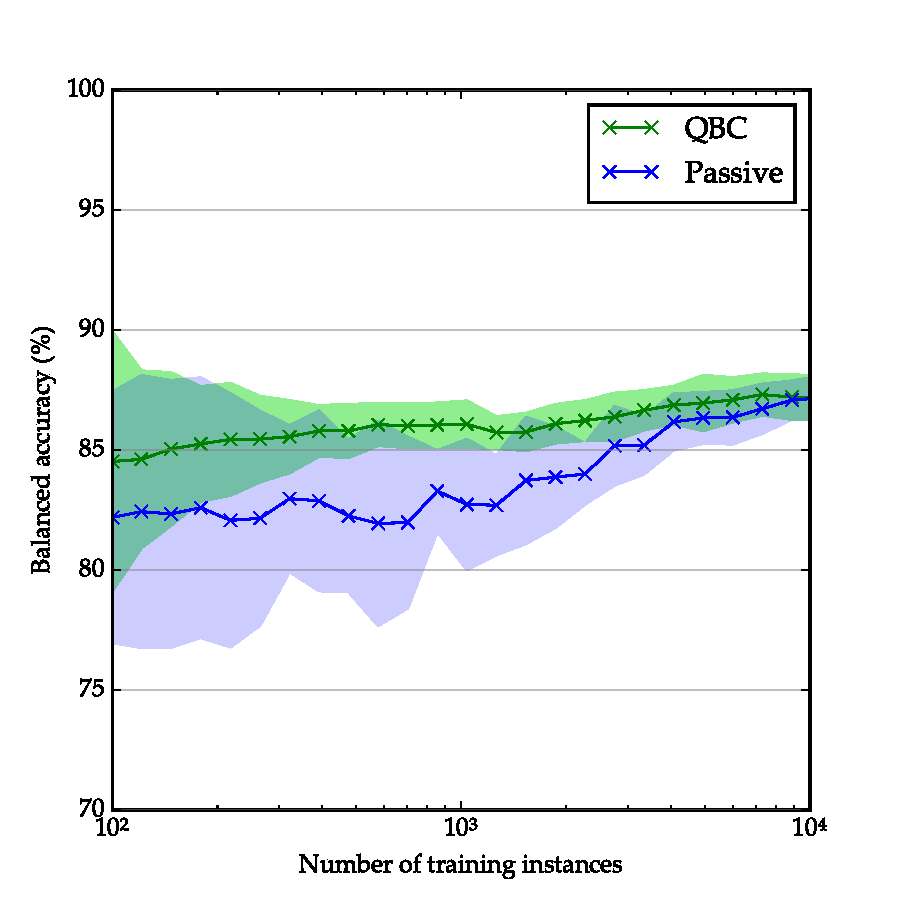
\includegraphics[width=0.8\textwidth]
            {images/experiments/rgz_qbc.pdf}
        \caption{Logistic regression trained on the \citeauthor{norris06}
            labels with different amounts of training data and two different
            query strategies.}
        \label{fig:rgz-qbc}
    \end{figure}

    We tested QBC active learning on the galaxy classification task described in
    Chapter \ref{cha:cross-identification}, comparing QBC to passive (i.e.
    random) selection as a query strategy.

    We used a committee of 20 logistic regression classifiers for the QBC test.
    Each was presented with 75\% of the known labels at random, stratified by
    the labels.

    For the passive test, we sampled 100 galaxies at random (stratified by the
    labels) and trained a logistic regression classifier on these. We then drew
    a batch of new labels, added these to the existing label set, and then
    retrained the classifier. This was repeated until the classifier had seen
    the entire training set ($10^4$ labels). The process for testing QBC was
    identical, except that instead of drawing new labels at random, the new
    labels were drawn in order of highest to lowest disagreement of the
    committee.

    After running the experiment, we observed that QBC outperformed passive
    selection. We hypothesised that this was because querying at random ignores
    the fact that there are far more negative examples than positive examples in
    the galaxy classification task. By this hypothesis, QBC would perform
    comparably to sampling from the set of positive examples and the set of
    negative examples at equal rates. To test this, we ran a third test with a
    random sampler that accounted for class imbalance. We found that this third
    test performed similarly to QBC.

    All three tested querying strategies are plotted in Figure
    \ref{fig:rgz-qbc}.

\section{Active Learning on Crowds}
\label{sec:active-learning-on-crowds}
    
    Traditional active learning assumes that we have access to one expert, who
    always issues correct labels. When labels are sourced from a crowd, these
    assumptions no longer hold: the crowd are non-experts and can give incorrect
    labels \citep{mozafari12,yan11}, and there are multiple labellers with
    different accuracies \citep{yan11}. We can now ask questions deeper than
    simply ``which label should I request?'' --- we can, for example, ask
    ``which labeller should I ask?'', or ``do I need to re-request this
    label?''.

    \citet{yan11} apply the \citet{yan10} model (Section \ref{sec:yan}) to the
    problem of active learning from crowds. We remind the reader that this model
    consists of a label model $p(z | \vec x)$ and a data-dependent labeller
    model $p(y_t | \vec x, z)$, where $\vec x$ is an instance, $y_t$ is the
    label assigned by labeller $t$, and $z$ is the groundtruth label. To extend
    this model into active learning, \citeauthor{yan11} introduce a query
    strategy where not only an instance is requested, but a specific labeller.

    First, uncertainty sampling is used with the label model to choose an ideal
    point to query. With logistic regression (Equation \ref{eq:raykar-logreg}),
    the decision boundary between positive and negative labels is a hyperplane
    $\vec w^T \vec x = 0$; uncertainty sampling would choose to query the point
    nearest (or on) this hyperplane. The labeller and instance to query are then
    chosen as solutions to the following optimisation problem:
    \begin{align*}
        \text{minimise}_{\vec x, t}\ & \eta_t(\vec x)\\
        \text{s.t. } & \vec w^T \vec x = 0.
    \end{align*}
    Intuitively, we query the instance on the decision hyperplane with the least
    noisy labeller. While this instance may not actually exist in our pool, we
    simply choose the instance closest to it (i.e. using Euclidean distance).

    This method has similar drawbacks to the \citeauthor{yan10} passive learning
    method described in Chapter \ref{cha:ml}: the number of parameters grows
    large with large numbers of annotators, and the expectation-maximisation
    algorithm only converges to a local minimum. In our implementation, training
    was also quite slow, meaning online active learning may be impractical. It
    also does not account for the possibility of relabelling instances.

    \citet{mozafari12} suggest an approach similar to uncertainty sampling, with
    uncertainty computed using a bootstrap method. A full description of this
    method is beyond the scope of this thesis. Instead, we look at the approach
    they take to handle noise. Noting that crowds may perform worse on some
    subsets of the data than other subsets, \citeauthor{mozafari12} solve an
    integer linear program to compute the redundancy required for different
    subsets of the instance pool. First, they partition the data, then estimate
    the probability of obtaining a correct crowd label for each partition. This
    estimation is accomplished by querying the crowd on a sample of instances
    from each partition. The estimated probability is then used to compute the
    redundancy required. For full details, we refer the reader to the paper
    \citep{mozafari12}.

\todo{Talk about citizen science and an ideal experiment}